\documentclass[twoside]{book}

% Packages required by doxygen
\usepackage{fixltx2e}
\usepackage{calc}
\usepackage{doxygen}
\usepackage[export]{adjustbox} % also loads graphicx
\usepackage{graphicx}
\usepackage[utf8]{inputenc}
\usepackage{makeidx}
\usepackage{multicol}
\usepackage{multirow}
\PassOptionsToPackage{warn}{textcomp}
\usepackage{textcomp}
\usepackage[nointegrals]{wasysym}
\usepackage[table]{xcolor}

% Font selection
\usepackage[T1]{fontenc}
\usepackage[scaled=.90]{helvet}
\usepackage{courier}
\usepackage{amssymb}
\usepackage{sectsty}
\renewcommand{\familydefault}{\sfdefault}
\allsectionsfont{%
  \fontseries{bc}\selectfont%
  \color{darkgray}%
}
\renewcommand{\DoxyLabelFont}{%
  \fontseries{bc}\selectfont%
  \color{darkgray}%
}
\newcommand{\+}{\discretionary{\mbox{\scriptsize$\hookleftarrow$}}{}{}}

% Page & text layout
\usepackage{geometry}
\geometry{%
  a4paper,%
  top=2.5cm,%
  bottom=2.5cm,%
  left=2.5cm,%
  right=2.5cm%
}
\tolerance=750
\hfuzz=15pt
\hbadness=750
\setlength{\emergencystretch}{15pt}
\setlength{\parindent}{0cm}
\setlength{\parskip}{3ex plus 2ex minus 2ex}
\makeatletter
\renewcommand{\paragraph}{%
  \@startsection{paragraph}{4}{0ex}{-1.0ex}{1.0ex}{%
    \normalfont\normalsize\bfseries\SS@parafont%
  }%
}
\renewcommand{\subparagraph}{%
  \@startsection{subparagraph}{5}{0ex}{-1.0ex}{1.0ex}{%
    \normalfont\normalsize\bfseries\SS@subparafont%
  }%
}
\makeatother

% Headers & footers
\usepackage{fancyhdr}
\pagestyle{fancyplain}
\fancyhead[LE]{\fancyplain{}{\bfseries\thepage}}
\fancyhead[CE]{\fancyplain{}{}}
\fancyhead[RE]{\fancyplain{}{\bfseries\leftmark}}
\fancyhead[LO]{\fancyplain{}{\bfseries\rightmark}}
\fancyhead[CO]{\fancyplain{}{}}
\fancyhead[RO]{\fancyplain{}{\bfseries\thepage}}
\fancyfoot[LE]{\fancyplain{}{}}
\fancyfoot[CE]{\fancyplain{}{}}
\fancyfoot[RE]{\fancyplain{}{\bfseries\scriptsize Generated by Doxygen }}
\fancyfoot[LO]{\fancyplain{}{\bfseries\scriptsize Generated by Doxygen }}
\fancyfoot[CO]{\fancyplain{}{}}
\fancyfoot[RO]{\fancyplain{}{}}
\renewcommand{\footrulewidth}{0.4pt}
\renewcommand{\chaptermark}[1]{%
  \markboth{#1}{}%
}
\renewcommand{\sectionmark}[1]{%
  \markright{\thesection\ #1}%
}

% Indices & bibliography
\usepackage{natbib}
\usepackage[titles]{tocloft}
\setcounter{tocdepth}{3}
\setcounter{secnumdepth}{5}
\makeindex

% Hyperlinks (required, but should be loaded last)
\usepackage{ifpdf}
\ifpdf
  \usepackage[pdftex,pagebackref=true]{hyperref}
\else
  \usepackage[ps2pdf,pagebackref=true]{hyperref}
\fi
\hypersetup{%
  colorlinks=true,%
  linkcolor=blue,%
  citecolor=blue,%
  unicode%
}

% Custom commands
\newcommand{\clearemptydoublepage}{%
  \newpage{\pagestyle{empty}\cleardoublepage}%
}

\usepackage{caption}
\captionsetup{labelsep=space,justification=centering,font={bf},singlelinecheck=off,skip=4pt,position=top}

%===== C O N T E N T S =====

\begin{document}

% Titlepage & ToC
\hypersetup{pageanchor=false,
             bookmarksnumbered=true,
             pdfencoding=unicode
            }
\pagenumbering{alph}
\begin{titlepage}
\vspace*{7cm}
\begin{center}%
{\Large Projeto 2 \\[1ex]\large 1.\+0 }\\
\vspace*{1cm}
{\large Generated by Doxygen 1.8.14}\\
\end{center}
\end{titlepage}
\clearemptydoublepage
\pagenumbering{roman}
\tableofcontents
\clearemptydoublepage
\pagenumbering{arabic}
\hypersetup{pageanchor=true}

%--- Begin generated contents ---
\chapter{Hierarchical Index}
\section{Class Hierarchy}
This inheritance list is sorted roughly, but not completely, alphabetically\+:\begin{DoxyCompactList}
\item \contentsline{section}{Point}{\pageref{class_point}}{}
\item \contentsline{section}{Poligono}{\pageref{class_poligono}}{}
\begin{DoxyCompactList}
\item \contentsline{section}{Retangulo}{\pageref{class_retangulo}}{}
\end{DoxyCompactList}
\end{DoxyCompactList}

\chapter{Class Index}
\section{Class List}
Here are the classes, structs, unions and interfaces with brief descriptions\+:\begin{DoxyCompactList}
\item\contentsline{section}{\mbox{\hyperlink{class_circulo}{Circulo}} \\*Desenha um círculo }{\pageref{class_circulo}}{}
\item\contentsline{section}{\mbox{\hyperlink{class_figura_geometrica}{Figura\+Geometrica}} }{\pageref{class_figura_geometrica}}{}
\item\contentsline{section}{\mbox{\hyperlink{class_reta}{Reta}} \\*Desenha uma reta }{\pageref{class_reta}}{}
\item\contentsline{section}{\mbox{\hyperlink{class_retangulo}{Retangulo}} \\*Desenha um retângulo }{\pageref{class_retangulo}}{}
\item\contentsline{section}{\mbox{\hyperlink{class_screen}{Screen}} \\*é a classe que define e tem a responsabilidade de configurar a tela de exibição ao usuário }{\pageref{class_screen}}{}
\end{DoxyCompactList}

\chapter{Class Documentation}
\hypertarget{class_circulo}{}\section{Circulo Class Reference}
\label{class_circulo}\index{Circulo@{Circulo}}


The \mbox{\hyperlink{class_circulo}{Circulo}} class desenha um círculo.  




{\ttfamily \#include $<$circulo.\+h$>$}

Inheritance diagram for Circulo\+:\begin{figure}[H]
\begin{center}
\leavevmode
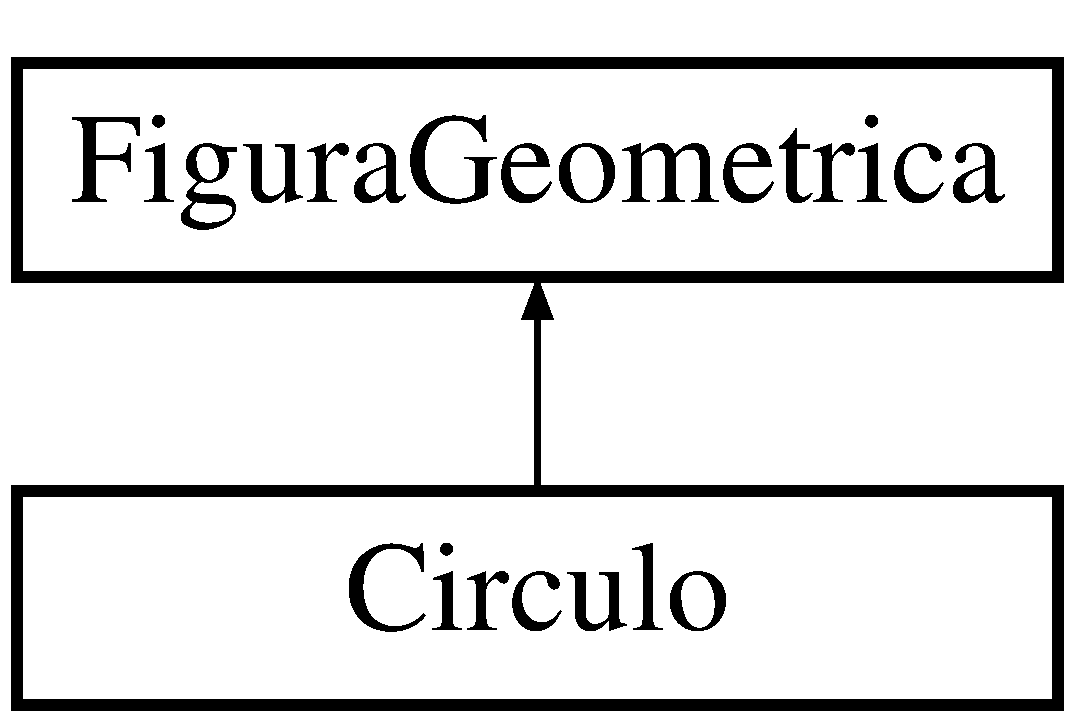
\includegraphics[height=2.000000cm]{class_circulo}
\end{center}
\end{figure}
\subsection*{Public Member Functions}
\begin{DoxyCompactItemize}
\item 
\mbox{\hyperlink{class_circulo_a5e0622e82a3ce86c9f7d247956bf98b3}{Circulo}} (float x0, float y0, float raio, float fillmode)
\begin{DoxyCompactList}\small\item\em \mbox{\hyperlink{class_circulo}{Circulo}} é o construtor da classe. \end{DoxyCompactList}\item 
void \mbox{\hyperlink{class_circulo_a593787d6e0618c2eded23e8839e7bea6}{draw}} (\mbox{\hyperlink{class_screen}{Screen}} \&t)
\begin{DoxyCompactList}\small\item\em draw é a função chave para desenhar a figura. \end{DoxyCompactList}\item 
void \mbox{\hyperlink{class_circulo_ac7946aa1d6e6a1290d123bdd542a2a90}{pontos\+Da\+Circunferencia}} (float x, float y, \mbox{\hyperlink{class_screen}{Screen}} \&t)
\begin{DoxyCompactList}\small\item\em pontos\+Da\+Circunferencia modifica de fato o valor da matriz nos pontos determinados pelo método draw. \end{DoxyCompactList}\end{DoxyCompactItemize}


\subsection{Detailed Description}
The \mbox{\hyperlink{class_circulo}{Circulo}} class desenha um círculo. 

Dentro da matriz que representa a tela, essa classe modifica posições específicas para que, quando colocado em um arquivo ou quando impresso em tela, forneça ao usuário um desenho de um disco ou de uma circunferência. 

\subsection{Constructor \& Destructor Documentation}
\mbox{\Hypertarget{class_circulo_a5e0622e82a3ce86c9f7d247956bf98b3}\label{class_circulo_a5e0622e82a3ce86c9f7d247956bf98b3}} 
\index{Circulo@{Circulo}!Circulo@{Circulo}}
\index{Circulo@{Circulo}!Circulo@{Circulo}}
\subsubsection{\texorpdfstring{Circulo()}{Circulo()}}
{\footnotesize\ttfamily Circulo\+::\+Circulo (\begin{DoxyParamCaption}\item[{float}]{x0,  }\item[{float}]{y0,  }\item[{float}]{raio,  }\item[{float}]{fillmode }\end{DoxyParamCaption})}



\mbox{\hyperlink{class_circulo}{Circulo}} é o construtor da classe. 


\begin{DoxyParams}{Parameters}
{\em x0} & é a posição fornecida pelo usuário, no eixo x, lido de um arquivo de texto. \\
\hline
{\em y0} & é a posição fornecida pelo usuário, no eixo x, lido de um arquivo de texto. \\
\hline
{\em raio} & é o raio fornecido pelo usuário a partir do arquivo de texto. \\
\hline
{\em fillmode} & é o valor (0 ou 1) fornecido pelo usuário para indicar se será desenhado um disco ou uma circunferência. \\
\hline
\end{DoxyParams}


\subsection{Member Function Documentation}
\mbox{\Hypertarget{class_circulo_a593787d6e0618c2eded23e8839e7bea6}\label{class_circulo_a593787d6e0618c2eded23e8839e7bea6}} 
\index{Circulo@{Circulo}!draw@{draw}}
\index{draw@{draw}!Circulo@{Circulo}}
\subsubsection{\texorpdfstring{draw()}{draw()}}
{\footnotesize\ttfamily void Circulo\+::draw (\begin{DoxyParamCaption}\item[{\mbox{\hyperlink{class_screen}{Screen}} \&}]{t }\end{DoxyParamCaption})\hspace{0.3cm}{\ttfamily [virtual]}}



draw é a função chave para desenhar a figura. 

Nela, o desenho da circunferência é feito usando o algoritmo de Bresenham para traçado de circunferências. Para os casos onde devemos preencher totalmente o círculo, fazemos com que todos os pontos que tivessem uma distância ao centro menor ou igual ao raio fossem preenchidos. Em outras palavras, usamos a inequação da circunferência para determinarmos quais pontos são internos ou pertencentes à ela (x$^\wedge$2+y$^\wedge$2 $<$= raio$^\wedge$2). 
\begin{DoxyParams}{Parameters}
{\em t} & é o endereço da matriz que representa a tela onde o círculo será desenhado. \\
\hline
\end{DoxyParams}


Implements \mbox{\hyperlink{class_figura_geometrica}{Figura\+Geometrica}}.

\mbox{\Hypertarget{class_circulo_ac7946aa1d6e6a1290d123bdd542a2a90}\label{class_circulo_ac7946aa1d6e6a1290d123bdd542a2a90}} 
\index{Circulo@{Circulo}!pontos\+Da\+Circunferencia@{pontos\+Da\+Circunferencia}}
\index{pontos\+Da\+Circunferencia@{pontos\+Da\+Circunferencia}!Circulo@{Circulo}}
\subsubsection{\texorpdfstring{pontos\+Da\+Circunferencia()}{pontosDaCircunferencia()}}
{\footnotesize\ttfamily void Circulo\+::pontos\+Da\+Circunferencia (\begin{DoxyParamCaption}\item[{float}]{x,  }\item[{float}]{y,  }\item[{\mbox{\hyperlink{class_screen}{Screen}} \&}]{t }\end{DoxyParamCaption})}



pontos\+Da\+Circunferencia modifica de fato o valor da matriz nos pontos determinados pelo método draw. 


\begin{DoxyParams}{Parameters}
{\em x} & representa a coluna que será modificada na matriz. \\
\hline
{\em y} & representa a linha que será modificada na matriz. \\
\hline
{\em t} & é a tela. \\
\hline
\end{DoxyParams}


The documentation for this class was generated from the following files\+:\begin{DoxyCompactItemize}
\item 
C\+:/\+Users/\+Dorgival/\+Desktop/\+Estudos/programacao\+\_\+avancada/\+Projeto2/circulo.\+h\item 
C\+:/\+Users/\+Dorgival/\+Desktop/\+Estudos/programacao\+\_\+avancada/\+Projeto2/circulo.\+cpp\end{DoxyCompactItemize}

\hypertarget{class_figura_geometrica}{}\section{Figura\+Geometrica Class Reference}
\label{class_figura_geometrica}\index{Figura\+Geometrica@{Figura\+Geometrica}}
Inheritance diagram for Figura\+Geometrica\+:\begin{figure}[H]
\begin{center}
\leavevmode
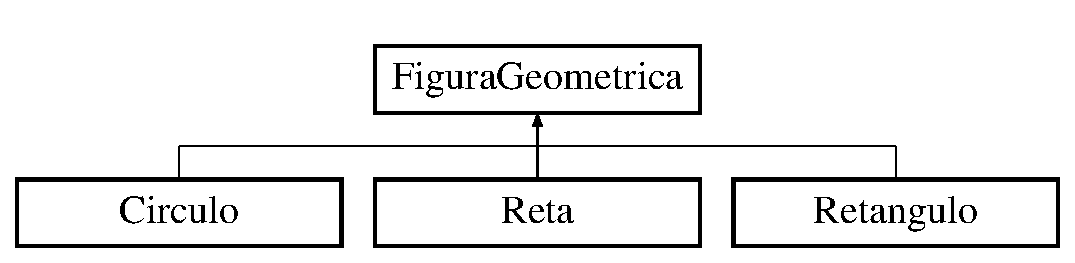
\includegraphics[height=2.000000cm]{class_figura_geometrica}
\end{center}
\end{figure}
\subsection*{Public Member Functions}
\begin{DoxyCompactItemize}
\item 
\mbox{\Hypertarget{class_figura_geometrica_a06404670d06d28d12f5f386901186925}\label{class_figura_geometrica_a06404670d06d28d12f5f386901186925}} 
virtual void {\bfseries draw} (\mbox{\hyperlink{class_screen}{Screen}} \&t)=0
\end{DoxyCompactItemize}


The documentation for this class was generated from the following files\+:\begin{DoxyCompactItemize}
\item 
C\+:/\+Users/\+Dorgival/\+Desktop/\+Estudos/programacao\+\_\+avancada/\+Projeto2/figurageometrica.\+h\item 
C\+:/\+Users/\+Dorgival/\+Desktop/\+Estudos/programacao\+\_\+avancada/\+Projeto2/figurageometrica.\+cpp\end{DoxyCompactItemize}

\hypertarget{class_reta}{}\section{Reta Class Reference}
\label{class_reta}\index{Reta@{Reta}}


The \mbox{\hyperlink{class_reta}{Reta}} class desenha uma reta.  




{\ttfamily \#include $<$reta.\+h$>$}

Inheritance diagram for Reta\+:\begin{figure}[H]
\begin{center}
\leavevmode
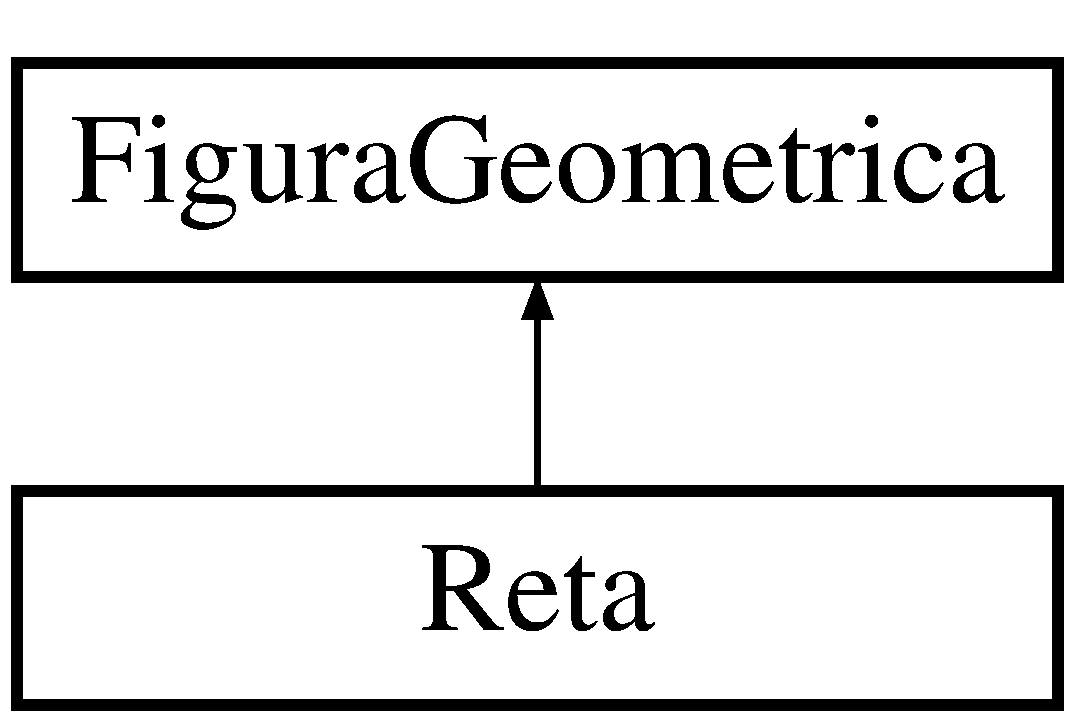
\includegraphics[height=2.000000cm]{class_reta}
\end{center}
\end{figure}
\subsection*{Public Member Functions}
\begin{DoxyCompactItemize}
\item 
\mbox{\hyperlink{class_reta_a9cde511ceb1d4e6638aaf735dfc24a7c}{Reta}} (float \+\_\+x0, float \+\_\+y0, float \+\_\+x1, float \+\_\+y1)
\begin{DoxyCompactList}\small\item\em \mbox{\hyperlink{class_reta}{Reta}} é o construtor da classe. \end{DoxyCompactList}\item 
void \mbox{\hyperlink{class_reta_ac2e9805183cd474b62bffd8b032cd780}{draw}} (\mbox{\hyperlink{class_screen}{Screen}} \&t)
\begin{DoxyCompactList}\small\item\em draw é a função chave para desenhar a figura. \end{DoxyCompactList}\end{DoxyCompactItemize}


\subsection{Detailed Description}
The \mbox{\hyperlink{class_reta}{Reta}} class desenha uma reta. 

Dentro da matriz que representa a tela, essa classe modifica posições específicas para que, quando colocado em um arquivo ou quando impresso em tela, forneça ao usuário um desenho de uma reta. 

\subsection{Constructor \& Destructor Documentation}
\mbox{\Hypertarget{class_reta_a9cde511ceb1d4e6638aaf735dfc24a7c}\label{class_reta_a9cde511ceb1d4e6638aaf735dfc24a7c}} 
\index{Reta@{Reta}!Reta@{Reta}}
\index{Reta@{Reta}!Reta@{Reta}}
\subsubsection{\texorpdfstring{Reta()}{Reta()}}
{\footnotesize\ttfamily Reta\+::\+Reta (\begin{DoxyParamCaption}\item[{float}]{\+\_\+x0,  }\item[{float}]{\+\_\+y0,  }\item[{float}]{\+\_\+x1,  }\item[{float}]{\+\_\+y1 }\end{DoxyParamCaption})}



\mbox{\hyperlink{class_reta}{Reta}} é o construtor da classe. 


\begin{DoxyParams}{Parameters}
{\em \+\_\+x0} & é o valor da posição inicial em x do ponto, fornecido pelo usuário. \\
\hline
{\em \+\_\+y0} & é o valor da posição inicial em y do ponto, fornecido pelo usuário. \\
\hline
{\em \+\_\+x1} & é o valor da posição final em x do ponto, fornecido pelo usuário. \\
\hline
{\em \+\_\+y1} & é o valor da posição final em y do ponto, fornecido pelo usuário. \\
\hline
\end{DoxyParams}


\subsection{Member Function Documentation}
\mbox{\Hypertarget{class_reta_ac2e9805183cd474b62bffd8b032cd780}\label{class_reta_ac2e9805183cd474b62bffd8b032cd780}} 
\index{Reta@{Reta}!draw@{draw}}
\index{draw@{draw}!Reta@{Reta}}
\subsubsection{\texorpdfstring{draw()}{draw()}}
{\footnotesize\ttfamily void Reta\+::draw (\begin{DoxyParamCaption}\item[{\mbox{\hyperlink{class_screen}{Screen}} \&}]{t }\end{DoxyParamCaption})\hspace{0.3cm}{\ttfamily [virtual]}}



draw é a função chave para desenhar a figura. 

Nela, o desenho da reta é feito usando o algoritmo de Bresenham para traçado de traços/retas. 
\begin{DoxyParams}{Parameters}
{\em t} & é o endereço da matriz que representa a tela onde a reta será desenhada. \\
\hline
\end{DoxyParams}


Implements \mbox{\hyperlink{class_figura_geometrica}{Figura\+Geometrica}}.



The documentation for this class was generated from the following files\+:\begin{DoxyCompactItemize}
\item 
C\+:/\+Users/\+Dorgival/\+Desktop/\+Estudos/programacao\+\_\+avancada/\+Projeto2/reta.\+h\item 
C\+:/\+Users/\+Dorgival/\+Desktop/\+Estudos/programacao\+\_\+avancada/\+Projeto2/reta.\+cpp\end{DoxyCompactItemize}

\hypertarget{class_retangulo}{}\section{Retangulo Class Reference}
\label{class_retangulo}\index{Retangulo@{Retangulo}}


The \mbox{\hyperlink{class_retangulo}{Retangulo}} é uma herdeira da classe \mbox{\hyperlink{class_poligono}{Poligono}}.  




{\ttfamily \#include $<$retangulo.\+h$>$}



Inheritance diagram for Retangulo\+:
% FIG 0


Collaboration diagram for Retangulo\+:
% FIG 1
\subsection*{Public Member Functions}
\begin{DoxyCompactItemize}
\item 
\mbox{\hyperlink{class_retangulo_acca1dd211eefc8dc04658c943c0d1122}{Retangulo}} (float x, float y, float largura, float altura)
\begin{DoxyCompactList}\small\item\em \mbox{\hyperlink{class_retangulo}{Retangulo}} é o construtor da classe. \end{DoxyCompactList}\end{DoxyCompactItemize}


\subsection{Detailed Description}
The \mbox{\hyperlink{class_retangulo}{Retangulo}} é uma herdeira da classe \mbox{\hyperlink{class_poligono}{Poligono}}. 

Como herdeira, ela tem todas as características de um polígono como o definido na classe herdade\+: convexo, número de vértices 3$<$=n$<$=100 e inteiramente dentro do plano cartesiano bidimensional. 

\subsection{Constructor \& Destructor Documentation}
\mbox{\Hypertarget{class_retangulo_acca1dd211eefc8dc04658c943c0d1122}\label{class_retangulo_acca1dd211eefc8dc04658c943c0d1122}} 
\index{Retangulo@{Retangulo}!Retangulo@{Retangulo}}
\index{Retangulo@{Retangulo}!Retangulo@{Retangulo}}
\subsubsection{\texorpdfstring{Retangulo()}{Retangulo()}}
{\footnotesize\ttfamily Retangulo\+::\+Retangulo (\begin{DoxyParamCaption}\item[{float}]{x,  }\item[{float}]{y,  }\item[{float}]{largura,  }\item[{float}]{altura }\end{DoxyParamCaption})}



\mbox{\hyperlink{class_retangulo}{Retangulo}} é o construtor da classe. 

Nele, temos a coordenada do canto inferior esquerdo do retângulo, sua largura e altura. Com isso, temos todas as informações necessárias para definir completamente um retângulo dentro no plano xy.


\begin{DoxyParams}{Parameters}
{\em x} & é a abscissa do vértice inferior esquerda do retângulo.\\
\hline
{\em y} & é a ordenada do vértice inferior esquerda do retângulo.\\
\hline
{\em largura} & é a largura do retângulo, em u.\+c.\\
\hline
{\em altura} & é a altura do retângulo, em u.\+c. \\
\hline
\end{DoxyParams}


The documentation for this class was generated from the following files\+:\begin{DoxyCompactItemize}
\item 
C\+:/\+Users/dorgi/\+Desktop/\+Estudos/programacao\+\_\+avancada/\+Projeto2/retangulo.\+h\item 
C\+:/\+Users/dorgi/\+Desktop/\+Estudos/programacao\+\_\+avancada/\+Projeto2/retangulo.\+cpp\end{DoxyCompactItemize}

\hypertarget{class_screen}{}\section{Screen Class Reference}
\label{class_screen}\index{Screen@{Screen}}


The \mbox{\hyperlink{class_screen}{Screen}} class é a classe que define e tem a responsabilidade de configurar a tela de exibição ao usuário.  




{\ttfamily \#include $<$screen.\+h$>$}

\subsection*{Public Member Functions}
\begin{DoxyCompactItemize}
\item 
\mbox{\hyperlink{class_screen_a6c21beca43d25854d8674445127ef2eb}{Screen}} (int \+\_\+nlin, int \+\_\+ncol)
\begin{DoxyCompactList}\small\item\em \mbox{\hyperlink{class_screen}{Screen}} é o construtor da classe. \end{DoxyCompactList}\item 
void \mbox{\hyperlink{class_screen_a88e90322ba2f1623b660c424be1c8f84}{set\+Tamanho}} (int \+\_\+nlin, int \+\_\+ncol)
\begin{DoxyCompactList}\small\item\em set\+Tamanho nos permite modificar o tamanho da tela. \end{DoxyCompactList}\item 
void \mbox{\hyperlink{class_screen_ae6bea81c57a22d226507c3c26fa95ee0}{set\+Pixel}} (int x, int y)
\begin{DoxyCompactList}\small\item\em set\+Pixel nos permite modificar o conteúdo do pixel. \end{DoxyCompactList}\item 
void \mbox{\hyperlink{class_screen_a35e74266b2a04e37b354ceff7a5f1031}{clear}} ()
\begin{DoxyCompactList}\small\item\em clear tem a função de limpar a tela. \end{DoxyCompactList}\item 
void \mbox{\hyperlink{class_screen_aebc4eb6cb5acf15a0f04c1494622ab23}{set\+Brush}} (char \+\_\+brush)
\begin{DoxyCompactList}\small\item\em set\+Brush determina qual será o caractere de desenho na tela. \end{DoxyCompactList}\end{DoxyCompactItemize}
\subsection*{Friends}
\begin{DoxyCompactItemize}
\item 
ostream \& \mbox{\hyperlink{class_screen_aab6a2880746bfe1b7964817cc8f0989e}{operator$<$$<$}} (ostream \&os, \mbox{\hyperlink{class_screen}{Screen}} \&t)
\begin{DoxyCompactList}\small\item\em operator $<$$<$ é a sobrecarga do operador $<$$<$ \end{DoxyCompactList}\end{DoxyCompactItemize}


\subsection{Detailed Description}
The \mbox{\hyperlink{class_screen}{Screen}} class é a classe que define e tem a responsabilidade de configurar a tela de exibição ao usuário. 

Nessa classe, uma matriz que representa a tela é criada, seu tamanho é modificável (set\+Tamanho), o caractere de desenho na tela é modificável(set\+Brush), o pixel na tela é modificável(set\+Pixel) e temos uma função para apagar toda a tela. 

\subsection{Constructor \& Destructor Documentation}
\mbox{\Hypertarget{class_screen_a6c21beca43d25854d8674445127ef2eb}\label{class_screen_a6c21beca43d25854d8674445127ef2eb}} 
\index{Screen@{Screen}!Screen@{Screen}}
\index{Screen@{Screen}!Screen@{Screen}}
\subsubsection{\texorpdfstring{Screen()}{Screen()}}
{\footnotesize\ttfamily Screen\+::\+Screen (\begin{DoxyParamCaption}\item[{int}]{\+\_\+nlin,  }\item[{int}]{\+\_\+ncol }\end{DoxyParamCaption})}



\mbox{\hyperlink{class_screen}{Screen}} é o construtor da classe. 


\begin{DoxyParams}{Parameters}
{\em nlin} & inicialização do número de linhas da matriz tela. \\
\hline
{\em ncol} & inicialização do número de colunas da matriz tela. \\
\hline
\end{DoxyParams}


\subsection{Member Function Documentation}
\mbox{\Hypertarget{class_screen_a35e74266b2a04e37b354ceff7a5f1031}\label{class_screen_a35e74266b2a04e37b354ceff7a5f1031}} 
\index{Screen@{Screen}!clear@{clear}}
\index{clear@{clear}!Screen@{Screen}}
\subsubsection{\texorpdfstring{clear()}{clear()}}
{\footnotesize\ttfamily void Screen\+::clear (\begin{DoxyParamCaption}{ }\end{DoxyParamCaption})}



clear tem a função de limpar a tela. 

Todas as posições da matriz recebem o char vazio\+: \textquotesingle{} \textquotesingle{} \mbox{\Hypertarget{class_screen_aebc4eb6cb5acf15a0f04c1494622ab23}\label{class_screen_aebc4eb6cb5acf15a0f04c1494622ab23}} 
\index{Screen@{Screen}!set\+Brush@{set\+Brush}}
\index{set\+Brush@{set\+Brush}!Screen@{Screen}}
\subsubsection{\texorpdfstring{set\+Brush()}{setBrush()}}
{\footnotesize\ttfamily void Screen\+::set\+Brush (\begin{DoxyParamCaption}\item[{char}]{\+\_\+brush }\end{DoxyParamCaption})}



set\+Brush determina qual será o caractere de desenho na tela. 

Ao selecionar um, todo o desenho será feito com ele, portanto, não será possível desenhar com dois brushs diferentes em um mesmo arquivo. 
\begin{DoxyParams}{Parameters}
{\em brush} & é um char que recebe o valor do usuário. \\
\hline
\end{DoxyParams}
\mbox{\Hypertarget{class_screen_ae6bea81c57a22d226507c3c26fa95ee0}\label{class_screen_ae6bea81c57a22d226507c3c26fa95ee0}} 
\index{Screen@{Screen}!set\+Pixel@{set\+Pixel}}
\index{set\+Pixel@{set\+Pixel}!Screen@{Screen}}
\subsubsection{\texorpdfstring{set\+Pixel()}{setPixel()}}
{\footnotesize\ttfamily void Screen\+::set\+Pixel (\begin{DoxyParamCaption}\item[{int}]{x,  }\item[{int}]{y }\end{DoxyParamCaption})}



set\+Pixel nos permite modificar o conteúdo do pixel. 

Dentro de uma posição específica da matriz, que seria o equivalente a trocar o valor do píxel na tela, esse método desenha um char, definido no \textquotesingle{}brush\textquotesingle{} como caractere de desenho. Quando selecionado um brush, todo o desenho será feito com ele. 
\begin{DoxyParams}{Parameters}
{\em x} & posição, em x, do pixel que será modificado. \\
\hline
{\em y} & posição, em y, do pixel que será modificado. \\
\hline
\end{DoxyParams}
\mbox{\Hypertarget{class_screen_a88e90322ba2f1623b660c424be1c8f84}\label{class_screen_a88e90322ba2f1623b660c424be1c8f84}} 
\index{Screen@{Screen}!set\+Tamanho@{set\+Tamanho}}
\index{set\+Tamanho@{set\+Tamanho}!Screen@{Screen}}
\subsubsection{\texorpdfstring{set\+Tamanho()}{setTamanho()}}
{\footnotesize\ttfamily void Screen\+::set\+Tamanho (\begin{DoxyParamCaption}\item[{int}]{\+\_\+nlin,  }\item[{int}]{\+\_\+ncol }\end{DoxyParamCaption})}



set\+Tamanho nos permite modificar o tamanho da tela. 

O que acontece de fato é a substituição na matriz antes preparada por outra na memória. Essa nova matriz pode ser menor, maior ou igual a anterior. Aqui, \+\_\+nlin e \+\_\+ncol devem ser maiores ou iguais a 0 
\begin{DoxyParams}{Parameters}
{\em \+\_\+nlin} & é a altura da tela. \\
\hline
{\em \+\_\+ncol} & é a largura da tela. \\
\hline
\end{DoxyParams}


\subsection{Friends And Related Function Documentation}
\mbox{\Hypertarget{class_screen_aab6a2880746bfe1b7964817cc8f0989e}\label{class_screen_aab6a2880746bfe1b7964817cc8f0989e}} 
\index{Screen@{Screen}!operator$<$$<$@{operator$<$$<$}}
\index{operator$<$$<$@{operator$<$$<$}!Screen@{Screen}}
\subsubsection{\texorpdfstring{operator$<$$<$}{operator<<}}
{\footnotesize\ttfamily ostream\& operator$<$$<$ (\begin{DoxyParamCaption}\item[{ostream \&}]{os,  }\item[{\mbox{\hyperlink{class_screen}{Screen}} \&}]{t }\end{DoxyParamCaption})\hspace{0.3cm}{\ttfamily [friend]}}



operator $<$$<$ é a sobrecarga do operador $<$$<$ 

A sobrecarga nos permite mostrar o desenho em tela ou gravar esse desenho em um arquivo. 
\begin{DoxyParams}{Parameters}
{\em os} & \\
\hline
{\em t} & é o endereço da matriz alocada. \\
\hline
\end{DoxyParams}
\begin{DoxyReturn}{Returns}

\end{DoxyReturn}


The documentation for this class was generated from the following files\+:\begin{DoxyCompactItemize}
\item 
C\+:/\+Users/\+Dorgival/\+Desktop/\+Estudos/programacao\+\_\+avancada/\+Projeto2/screen.\+h\item 
C\+:/\+Users/\+Dorgival/\+Desktop/\+Estudos/programacao\+\_\+avancada/\+Projeto2/screen.\+cpp\end{DoxyCompactItemize}

%--- End generated contents ---

% Index
\backmatter
\newpage
\phantomsection
\clearemptydoublepage
\addcontentsline{toc}{chapter}{Index}
\printindex

\end{document}
